\begin{figure}[htbp]
    \centering
    \scalebox{1}{
    \begin{minipage}{0.48\textwidth}
        \centering
        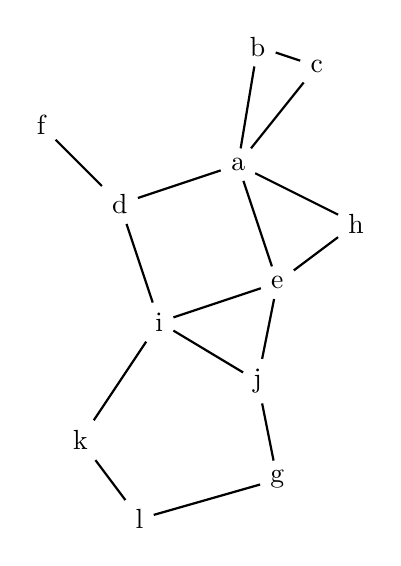
\begin{tikzpicture}[thick]
            % Nodes with manual coordinates
            \node (a) at (0.5,-1.5) {a};
            \node (b) at (0.75,0) {b};
            \node (c) at (1.5,-0.25) {c};
            \node (d) at (-1,-2) {d};
            \node (e) at (1,-3) {e};
            \node (f) at (-2,-1) {f};
            \node (g) at (1,-5.5) {g};
            \node (h) at (2,-2.25) {h};
            \node (i) at (-0.5,-3.5) {i};
            \node (j) at (0.75, -4.25) {j};
            \node (k) at (-1.5,-5) {k};
            \node (l) at (-0.75,-6) {l};
            
            % Edges
            \draw (a) -- (b);
            \draw (a) -- (c);
            \draw (a) -- (d);
            \draw (a) -- (e);
            \draw (b) -- (c);
            \draw (e) -- (j);
            \draw (e) -- (h);
            \draw (d) -- (i);
            \draw (d) -- (f);
            \draw (j) -- (g);
            \draw (i) -- (j);
            \draw (i) -- (e);
            \draw (i) -- (k);
            \draw (g) -- (l);
            \draw (h) -- (a);
            \draw (l) -- (k);
        \end{tikzpicture}
        \label{fig:graph}
    \end{minipage}
    \hfill
    % Second graph (formerly tree layout)
    \begin{minipage}{0.48\textwidth}
        \centering
        \begin{tikzpicture}[thick]
            % Tree nodes
            \node (e) at (0,0) {$e$};
            \node (i) at (0,-1.5) {$i$};
            \node (a) at (-1.5,-3) {$a$};
            \node (g) at (1.5,-3) {$g$};
            \node (c) at (-2.5,-4.5) {$c$};
            \node (h) at (-1.5,-4.5) {$h$};
            \node (f) at (-0.5,-4.5) {$f$};
            \node (j) at (1,-4.5) {$j$};
            \node (k) at (2,-4.5) {$k$};
            \node (b) at (-3,-6) {$b$};
            \node (d) at (-0.5,-6) {$d$};
            \node (l) at (2,-6) {$l$};

            % Edges
            \draw[->] (e) -> (i);
            \draw[->] (i) -- (a);
            \draw[->] (i) -- (g);
            \draw[->] (a) -- (c);
            \draw[->] (a) -- (h);
            \draw[->] (a) -- (f);
            \draw[->] (c) -- (b);
            \draw[->] (f) -- (d);
            \draw[->] (g) -- (j);
            \draw[->] (g) -- (k);
            \draw[->] (k) -- (l);
        \end{tikzpicture}
    \end{minipage}
    \caption[Graph and a decision tree for it]{Sample input graph (on the left) and a decision tree for it (on the right).}
    \label{fig:sample_decision_trees_for_graph}}
\end{figure}
